\documentclass{article}
\usepackage{ctex}
\usepackage{amsmath}

\title{计算机图形学第三次实验}
\author{陈小羽 2016060106020}
\date{}

\begin{document}
\maketitle

\section{实验名称}
	\paragraph{}
		画笔软件原型设计与开发
\section{实验内容和目的}
	\subsection{实验目的}
		\paragraph{}
			通过巩固所学的图形学方面的基本知识,了解和掌握
			图形交互系统设计方法和技能
	\subsection{实验内容}
		\paragraph{}
			设计实现一个简单的交互式画笔软件
	\subsection{基本要求}
		\paragraph{}
			\begin{itemize}
				\item 支持矩形绘制、多边形绘制、圆绘制、椭圆绘制
				\item 支持Bezier曲线绘制,鼠标输入控制点
				\item 支持图形填充
				\item 程序能正常退出
			\end{itemize}

\section{实验原理}
	\paragraph{}
		通过使用OpenGL提供的glDrawPixels()函数, 我们可以将一个二进制数组
		直接写入窗口中的特定位置. 所以, 所有的绘图操作现在转化为了对于
		数组中元素的读写操作.
	\paragraph{}
		问题转化之后, 我们就可以很容易的使用书上讲到的各种画线, 画圆和填充
		算法来实现一些画图软件基本的功能.
	\paragraph{}
		有了绘制图元的算法之后, 我们可以使用这些自己打包好的算法来绘制一个
		简单的图形界面, 来实现与用户的交互.
	\paragraph{}
		对于一些原理的细节(比如画线算法), 会在实验步骤中提到, 这里就不写了, 免得
		重复.

\section{实验器材(设备, 元器件)}
	\begin{center}
		\begin{tabular}{|c|c|}
			\hline
			系统 & macOS 10.13.1 \\
			\hline
			处理器 & 2GHz Intel Core i5 \\
			\hline 
			内存 & 8GB 1867 MHz LPDDR3 \\
			\hline 
			图形卡 & Intel Iris Graphics 540 1536MB \\
			\hline
		\end{tabular}
	\end{center}
\section{实验步骤和结果分析}
	\subsection{Paper类型}
		\paragraph{}
			因为我需要自己实现所有的画线算法, 所以我首先实现了一个比较底层的类型.
			Paper类型的主要作用是维护一个数组, 这个数组在这里可以认为是显存(画布).
			然后这个类型提供了一些功能:
			\begin{itemize}
				\item 对于某一个坐标上的像素的读写(计算偏移量)
				\item 用某一种颜色清空缓冲区
				\item 绘制过程中对越界行为的处理
				\item 整体移动画布的位置
				\item 更改画布的大小
			\end{itemize}
	\subsection{Pen类型}
		\paragraph{}
			这个类型是为了对Paper类型的功能做进一步的封装. 可以用于记录
			每个物体各自的颜色和绘制时的一些细节(比如有些算法在绘制的时候要求
			对颜色的混合).
	\subsection{算法模板类型}
		\paragraph{}
			我在这个类型中统一打包了绘图程序中用到的所有绘图的算法.	
		\subsubsection{Bresenham画线算法}
			\paragraph{}
				Bresenham画线算法被封装在LineAlgorithm类型中.
				这个算法通过将原来DDA算法进行了一些推广. 在直线的斜率
				$k \in [0, 1]$时每次将横坐标$x$加一, 然后通过一个判别式
				来判断纵坐标$y$是否需要加一(这个算法的细节部分可以参考课本).
			\paragraph{}
				最后, 根据对称性, 我们可以将这个算法推广到所有可能的斜率.
				具体的实现可以在LineAlgorithm.h中的LineBresenhamAlgorithm()
				中查看. 我的实现和书上的长度差不多, 但是却能支持所有的斜率.
		\subsubsection{吴小林画线算法}
			\paragraph{}
				因为Bresenham画线算法绘制出来的线条大都带有锯齿, 
				所以我在LineAlgorithm类型中加入了另一个绘制直线的算法. 
				这个算法是吴小林发明的, 所以一般被称作吴小林画线算法.
				这个算法在1991年上被吴在<<An efficient antialiasing 
				technique>> 上提出
			\clearpage
			\paragraph{idea}
				\begin{center}
					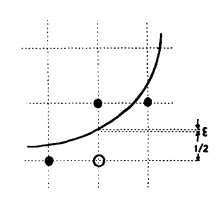
\includegraphics[width = 5cm]{wu-idea.jpeg} \\
				\end{center}
				从这个图中可以看到, Bresenham算法在处理中间那两个点的
				情况的时候, 根据实现, 只会选择两个点中的一个. 这样,
				如果选这了上面的那个点, 就会导致我们绘制出来的图形看起来
				不太平滑. 为了解决这个问题, 我们可以同时绘制两个点. 
				然后保证两个点的亮度之和为1. 比如, 如果我们要绘制$(x, f(x))$
				这个点. 我们就可以同时绘制$(x, \lfloor f(x) \rfloor)$和
				$(x, \lceil f(x) \rceil)$这两个点. 并且亮度分别为:
				$\lceil f(x) \rceil - f(x)$和$f(x) - \lfloor f(x) \rfloor$, 
				相当于这个点离$(x, f(x))$越近, 这个点就越亮. 最后看上去, 
				$(x, f(x))$就好像真的被绘制在屏幕上了一样.
				下面是放大之后的效果图.
				\begin{center}
					
\includegraphics[width = 5cm]{wu-draw.jpeg} \\
				\end{center}
			\paragraph{实现1}
				这个算法在实现的时候可以说是十分巧妙了.
				实现这个算法需要手动维护一个整数$D$. 
				$D$实际代表了一个小于1的定点小数$f$, 而且有如下关系
				$D = 2^{31}f$. $D$的最高位用于检测$D$是否溢出.
				假设斜率为$0 \leq k \leq 1$, 则按照DDA的流程, 我们
				可以每次使得$D = D + 2^{31}k$, 如果$D$溢出的话, 说明
				这个时候纵坐标$y$应该加一了, 否则$y$不变.
			\paragraph{实现2}
				更加好的是, 我们还可以同时使用这个$D$来维护上下两个点的亮度,
				我们可以取$D$的最高的8位作为$(x, \lceil f(x) \rceil)$这个点的
				亮度参考值(最大设置为255), 不妨设为$l$. 则另外一个点的亮度参考值
				就为$\bar{l}$(相当于按位取反操作). 可以这么做是因为$D$的最高8位
				相当于$(f(x) - \lfloor f(x) \rfloor) \times 2^8$, 这恰恰就是
				我们上面讨论出来上面的那个点需要的亮度值.
		\subsubsection{中点画圆和吴小林画圆算法算法}
			\paragraph{}
				画圆的算法和画线的算法基本上是相同的套路, 基本上也是每次
				$x = x + 1$, 然后这个时候使用一个判别式来判断这个时候$y$
				是不是应该减一(第一象限上半部分), 最后使用对称性补全这个
				图形中的其他的部分.
		\subsubsection{椭圆绘制算法}
			\paragraph{}
				椭圆的绘制我没有使用书上的公式, 主要使用的是椭圆的参数方程
				做的近似, 然后使用画线算法绘制的. 这样子可以做到使用3个控制
				点来控制椭圆, 可以绘制出长轴和短轴不平行与坐标轴的椭圆.
		\subsubsection{填充算法}
			\paragraph{}
				填充算法我只实现了洪泛填充. 最开始书上介绍了一种基于深度
				优先搜索的写法, 但是他没有考虑到这种写法容易爆栈. 所以
				我稍微做了一下改进, 用队列实现的相同的功能, 而且我没有
				使用递归, 我的程序应该没有调用函数的开销, 应该会跑得快一些.
		\subsubsection{Bezier曲线绘制算法}
			\paragraph{}
				贝塞尔曲线的绘制也是十分简单的, 只需要将书上的公式抄一遍,
				就完成了编写.
	\section{界面类型}
		\paragraph{}
			有了绘制图形的各种算法之后, 我制作了绘制图形的各种功能. 
			并且, 除此之外, 我还制作了简易的交互系统. 有了这个简易的交互
			系统之后, 用户可以调整颜色, 选择一些图形并进行操作. 
			下面将单独介绍这些功能.
		\subsubsection{关键点类型}
			\paragraph{}
				我写的画板程序使用的是矢量图形, 虽然我没有去实现放缩,
				平移和旋转的功能, 但是我在图形的表示方式这个问题上却
				是参考的矢量图形的标准. 在这个程序中, 所有的图元都是
				通过绑定在一些关键点上从而进行绘制的. 
			\paragraph{}
				用户在绘制图形的时候可以使用之前已经存在的关键点, 也
				可以添加新的关键点. 由于关键点和图元是分开维护的, 他们
				之间只使用指针传递信息. 所以, 在绘制完成之后, 用户
				仍然可以使用鼠标拖动关键点来实现对图元的控制.
			\paragraph{}
				考虑到关键点有可能会遮挡住绘制的图, 所以当按下h键的时候
				会停止绘制所有的关键点(隐藏).
		\subsubsection{选择功能}
			\paragraph{}
				因为需要添加擦子和更改颜色的功能, 这些后续功能都需要
				知道用户想对那一个图元进行操作. 所以这就需要一个用于
				选择的功能. 
			\paragraph{}
				选择功能能够在菜单之中找到, 使用之后拖动鼠标就可以在屏幕
				上看到一个红色的框, 被框中的关键点会被选中(变为绿色).
				为了应对有一些情况, 我对于直接点击某一个关键点的行为做了
				特判, 这样也是可以进行选择的.
			\paragraph{}
				考虑到有可能需要多选, 所以我设置了a键作为多选的开关.
				按下a键之后会开启多选功能.
			\paragraph{}
				在选择完成过后, 用户再次点击鼠标是不会取消选择或者选中新的
				关键点的. 也就是说选择操作是和其他的操作独立的. 
			\paragraph{}
				后续的功能在选择之后进行. 根据我的设计, 我使用如下的策略
				来判断到底那一个图元被选中了:
				\begin{itemize}
					\item 如果一个图元的所有的关键点都被选中了, 那么这个
					      图元被选中了.
					\item 如果有多个图元满足上个条件, 那么去最早创建
					      的图元作为被选中的图元.
				\end{itemize}
		\subsubsection{擦子}
			\paragraph{}
				这个功能实现出来是用来作为这个绘图程序的橡皮擦的. 因为这个
				程序是矢量绘图程序, 所以不能使用常规意义上的那种橡皮擦, 
				所以, 这个功能的代替就是删除操作. 这个程序可以支持删除
\end{document}
